
% This LaTeX was auto-generated from MATLAB code.
% To make changes, update the MATLAB code and republish this document.

\documentclass{article}
\usepackage{graphicx}
\usepackage{color}

\sloppy
\definecolor{lightgray}{gray}{0.5}
\setlength{\parindent}{0pt}

\begin{document}

    
    

\section*{Q4 c}

\begin{par}
\begin{verbatim}include>forward_A.m</include\end{verbatim} \begin{verbatim}include>cgconvtik.m</include\end{verbatim}
\end{par} \vspace{1em}
\begin{verbatim}
addpath("autoArrangeFigures");
close all; clc; clear;
X = double(imread('cameraman.tif'));
H = gauss2d(15,15,0,0,2,2);
D1 = [-1 0 1]';
D2 = D1';

Y = conv2(X,H,'same');
sigma_s = var(Y(:));
sigma_n = sigma_s * 1e-3;
noise = sigma_n * randn(size(Y));
Y = Y + noise;
n_iter = 500;
x_0 = X;
for lambda = power(10,linspace(-2,log10(20),20))
    estimate = cgconvtik(H, D1, D2, Y, x_0, lambda, n_iter);
    figure
    X_back = reshape(estimate,size(X));
    imagesc(normalize(X_back,'range')), colormap gray
    title({['\lambda = ',num2str(lambda)], ['N_{iter} = ',num2str(n_iter)]})
end
autoArrangeFigures(4,5,1)
\end{verbatim}

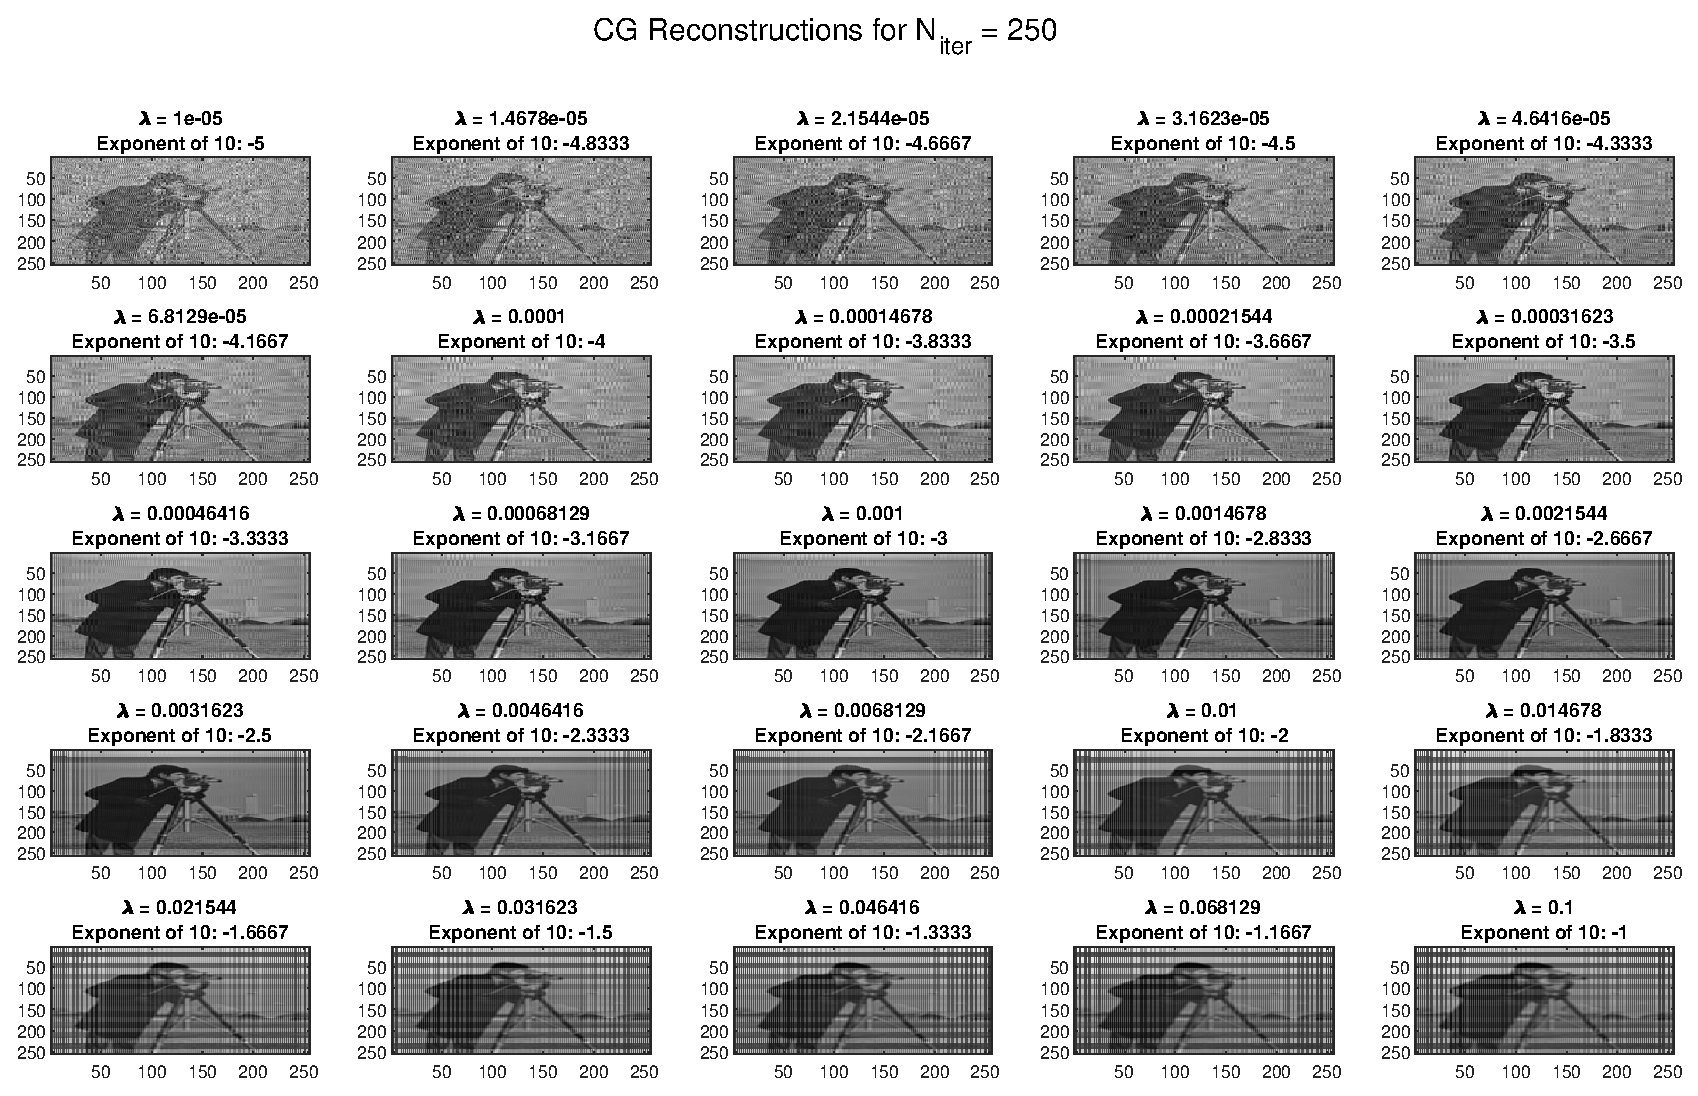
\includegraphics [width=4in]{Q4_01.eps}

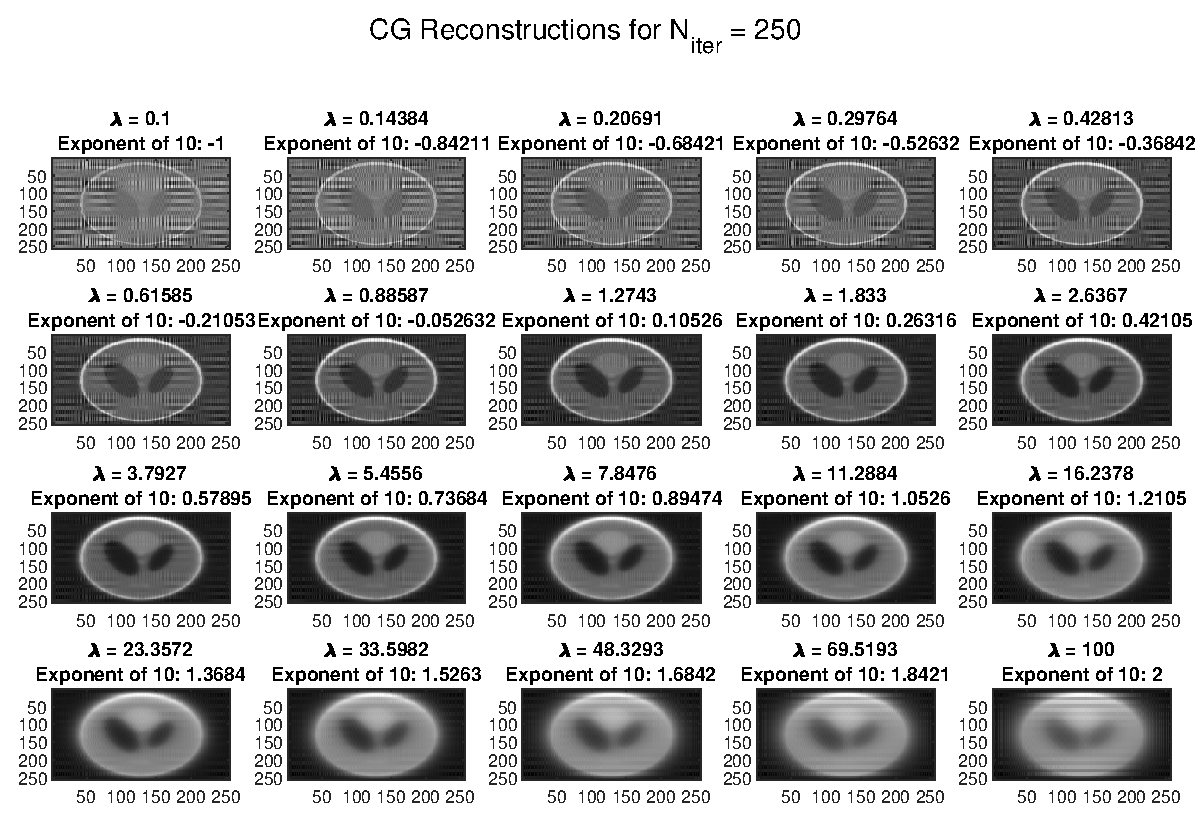
\includegraphics [width=4in]{Q4_02.eps}

\includegraphics [width=4in]{Q4_03.eps}

\includegraphics [width=4in]{Q4_04.eps}

\includegraphics [width=4in]{Q4_05.eps}

\includegraphics [width=4in]{Q4_06.eps}

\includegraphics [width=4in]{Q4_07.eps}

\includegraphics [width=4in]{Q4_08.eps}

\includegraphics [width=4in]{Q4_09.eps}

\includegraphics [width=4in]{Q4_10.eps}

\includegraphics [width=4in]{Q4_11.eps}

\includegraphics [width=4in]{Q4_12.eps}

\includegraphics [width=4in]{Q4_13.eps}

\includegraphics [width=4in]{Q4_14.eps}

\includegraphics [width=4in]{Q4_15.eps}

\includegraphics [width=4in]{Q4_16.eps}

\includegraphics [width=4in]{Q4_17.eps}

\includegraphics [width=4in]{Q4_18.eps}

\includegraphics [width=4in]{Q4_19.eps}

\includegraphics [width=4in]{Q4_20.eps}



\end{document}

